\section{Experiments}
\label{sec:experiments}

\subsection{Setup Recap}
Each fold trains one encoder on pooled source-normal windows (3 seeds, 4000 steps) and evaluates all four calibration mechanisms post hoc on the same scores and divergence traces, at nominal levels $\alphaNom\in\{0.05,0.10,0.20,0.30\}$. This design isolates the calibration layer: training is independent of the thresholding mechanism, so differences between mechanisms are not confounded by retraining. Evaluation windows per fold are listed in Table~\ref{tab:datasets}; labels and protocols per Section~\ref{sec:protocols}.

\subsection{Static Thresholds Fail in Both Directions; ACI Restores Coverage}
Table~\ref{tab:main} reports normal-window coverage at $\alphaNom=0.10$ (nominal $0.90$) and the mean coverage gap across the four nominal levels, averaged over seeds. Static source thresholds fail on every fold, and the failures are not small: on F2 (wind) coverage collapses to $0.18$---the source threshold over-alarms normal operation almost constantly---while the other five folds sit at $0.989$--$0.999$, i.e., the threshold is too high and alarms almost never fire. A single source-calibrated number is thus not merely imprecise; it is unusable in practice in opposite directions on different target domains.

Online ACI repairs this on five of six folds: mean gaps of $0.006$--$0.015$ (F1, F2, F4, F5, F6) against $0.077$--$0.523$ for static. Under moving-block bootstrap (seed~0, $\alphaNom{=}0.10$, 400 resamples), the ACI coverage interval stays within $\pm0.02$ of nominal for F1/F2/F4/F5 at moderate-to-long blocks, while F6 widens with block length (up to $[0.897,0.933]$ at $L{=}1{,}000$)---consistent with its slow drift---and F3 remains the synthetic exception. Averages are robust to weighting: macro versus window-weighted (micro) mean ACI gaps at $\alphaNom{=}0.10$ are $0.022$ vs $0.012$ (NA-ACI: $0.021$ vs $0.011$). The one exception is F3 (solar, synthetic injection): every mechanism stays at coverage $\approx 0.998$. This is the alarm-budget effect defined in Section~\ref{sec:setup-metrics}: F3's evaluation windows contain 20\% strongly separable injected anomalies, and once ACI has spent the alarm budget on them (87\% of injected runs detected, median delay 0), the normal-window FPR is driven to nearly zero. Coverage on F3 therefore over-shoots, and we read F3 as a synthetic-anomaly stress case rather than a calibration success. Figure~\ref{fig:coverage} shows the full $\alphaNom$-sweep; the nominal line is tracked on five folds and missed on F3 for the stated reason.

\begin{table}[t]
\caption{Normal-window coverage at $\alphaNom{=}0.10$ (nominal 0.90, mean of 3 seeds), per-fold AUROC and AUPRC, and mean coverage gap across $\alphaNom\in\{0.05,0.10,0.20,0.30\}$. Best per row in bold. $\dagger$ below-chance ranking: excluded from detection-quality claims. $\ddagger$ synthetic-only fold (F3); its over-coverage stems from the alarm budget being consumed by separable injected anomalies. Cross-variant differences within seed spread are not claimed as significant (descriptive comparisons only; three seeds).}
\label{tab:main}
\centering
\small
\resizebox{\columnwidth}{!}{%
\begin{tabular}{lcccccccc}
\toprule
 & & & \multicolumn{4}{c}{Coverage @ 0.10} & \multicolumn{2}{c}{Mean gap} \\
\cmidrule(lr){4-7}\cmidrule(lr){8-9}
Fold & AUROC & AUPRC & Static & ACI & Shift & Mondrian & Static & ACI \\
\midrule
F1 & 0.63 & 0.152 & 0.989 & 0.899 & 0.899 & 0.911 & 0.077 & \textbf{0.009} \\
F2$^\dagger$ & 0.39 & 0.099 & 0.183 & 0.890 & 0.890 & 0.871 & 0.523 & \textbf{0.010} \\
F3$^\ddagger$ & 0.79 & 0.728 & 0.999 & 0.998 & 0.998 & 0.999 & 0.160 & 0.105 \\
F4 & 0.99 & 0.992 & 0.999 & 0.910 & 0.908 & 0.920 & 0.160 & \textbf{0.010} \\
F5$^\dagger$ & 0.37 & 0.725 & 0.994 & 0.899 & 0.899 & 0.904 & 0.351 & \textbf{0.006} \\
F6 & 0.78 & 0.682 & 0.998 & 0.915 & 0.915 & 0.929 & 0.082 & \textbf{0.015} \\
\bottomrule
\end{tabular}}
\end{table}

\begin{figure*}[t]
\centering
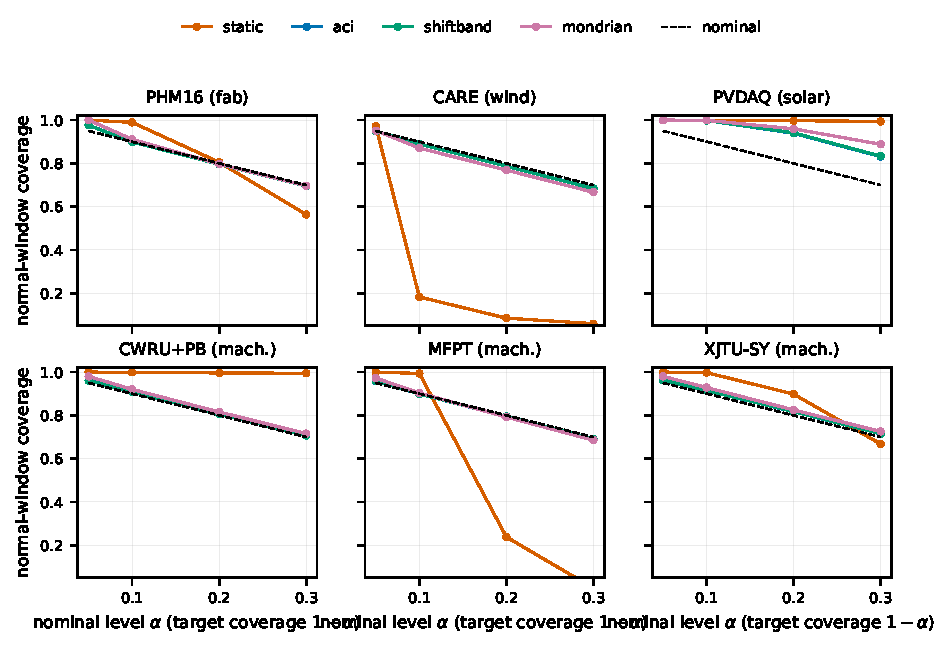
\includegraphics[width=\textwidth]{fig_coverage_alpha.pdf}
\caption{Normal-window coverage versus nominal level $\alphaNom$ per fold (mean over seeds). Dashed line: nominal $1-\alphaNom$. Static thresholds fail in both directions; ACI tracks the nominal level on five folds. F3 (injected synthetic anomalies) over-covers because the alarm budget is consumed by separable anomalies.}
\label{fig:coverage}
\end{figure*}

\subsection{The Alarm-Budget Defect and NA-ACI}
\label{sec:na-aci-results}
On anomaly-rich folds, plain ACI spends its alarm budget on anomalies and over-covers normal windows: at $\alphaNom{=}0.10$, F3's normal-window FPR is $0.002$ (ACI detects 39\% of injected anomalies), F4's anomaly detection rate is only $0.12$ while its FPR sits at the nominal $0.09$, and F6 detects $19\%$. Normal-anchored ACI (Section~\ref{sec:na-aci}) reallocates the budget: with $\kappa{=}3$, F4 detection rises to $0.90$ at FPR $0.094$, F6 to $0.29$ at $0.094$, F3 to $0.51$ at $0.026$, and F5 from $0.11$ to $0.16$ detection at unchanged FPR. Table~\ref{tab:na} summarizes calibration gaps, FPR, detection rates, and range-$F_1$. Across all folds and nominal levels, mean range-$F_1$ improves from $0.265$ (ACI) to $0.389$ ($\kappa{=}3$; $0.370$ at $\kappa{=}5$) while the mean coverage gap stays comparable ($0.026$ vs.\ $0.029$ at $\kappa{=}3$, and improves to $0.020$ at $\kappa{=}5$); anomaly-sparse folds F1/F2 are unchanged at $\kappa{=}5$ and mildly worse at $\kappa{=}3$ (F2 gap $0.010\!\to\!0.058$), exposing the expected $\kappa$ trade-off: aggressive exclusion risks excluding normal windows during scale drift and over-alarms. $\kappa$ is the method's only new hyper-parameter and can be validated online by monitoring the exclusion rate; we default to $\kappa{=}5$ when anomaly prevalence is low or unknown, $\kappa{=}3$ when prevalence is high.

\emph{Temporal diagnosis of the defect.} Mean coverage hides the dynamics. On F4 and F6 the ACI threshold traces show a limit cycle: the 5th--95th percentile range of the deployed threshold spans $0.005$--$2.0$ (F4) and $0.014$--$2.8$ (F6)---two to three orders of magnitude---with thousands of oscillation events per stream. The mechanism is integral windup: on anomaly-rich streams the alarm indicator stays on, the relative-gain integrator pushes the threshold up until the stream falls silent, the threshold then decays back, and the cycle repeats---alarm bursts alternate with long blind stretches (F4: longest alarm-free run $491$--$579$ windows, essentially all of it consecutive missed anomalies; F6: $\approx 1400$-window silences containing $338$--$346$ consecutive missed anomalies). Plain ACI on F4 thus shows FPR $0.090$ with detection only $0.118$ despite AUROC $0.99$: the time-averaged calibration looks nominal while the detector alternates between blindness and bursts, which is how those three numbers coexist. NA-ACI breaks the cycle by construction: with $\kappa{=}3$ the longest consecutive miss streak falls from $491$--$579$ to $51$--$106$ on F4 and from $\approx 340$ to $36$--$46$ on F6, and detection rises to $0.88$--$0.92$ and $0.29$, respectively. We therefore read the alarm-budget defect as two mechanisms---budget consumption by separable anomalies (F3-type, over-coverage) and windup-induced blindness (F4/F6-type)---both removed by excluding likely-anomalous windows from the feedback path; in control terms, the exclusion acts as anti-windup on the quantile integrator.

\begin{table}[t]
\caption{Alarm-budget defect and NA-ACI at $\alphaNom{=}0.10$ (3 seeds). Mean gap is over four nominal levels. NA-ACI reallocates alarms to anomalies (columns Det.) at essentially unchanged normal-window FPR, with large range-$F_1$ gains on anomaly-rich folds; $\kappa{=}3$ is aggressive, $\kappa{=}5$ conservative.}
\label{tab:na}
\centering
\small
\resizebox{\columnwidth}{!}{%
\begin{tabular}{lcccccccc}
\toprule
 & \multicolumn{2}{c}{ACI} & \multicolumn{3}{c}{NA-ACI $\kappa{=}3$} & \multicolumn{3}{c}{NA-ACI $\kappa{=}5$} \\
\cmidrule(lr){2-3}\cmidrule(lr){4-6}\cmidrule(lr){7-9}
Fold & FPR/Det. & R-$F_1$ & FPR/Det. & gap & R-$F_1$ & FPR/Det. & gap & R-$F_1$ \\
\midrule
F1 & .101/.065 & 0.07 & .105/.066 & 0.060 & 0.07 & .102/.065 & 0.012 & 0.07 \\
F2$^\dagger$ & .110/.136 & 0.13 & .137/.159 & 0.058 & 0.14 & .124/.148 & 0.031 & 0.14 \\
F3$^\ddagger$ & .002/.389 & 0.56 & .026/.512 & 0.044 & 0.63 & .019/.506 & 0.058 & 0.64 \\
F4 & .090/.118 & 0.19 & .094/.895 & 0.005 & 0.88 & .092/.715 & 0.006 & 0.77 \\
F5$^\dagger$ & .101/.106 & 0.19 & .101/.158 & 0.006 & 0.26 & .101/.138 & 0.006 & 0.24 \\
F6 & .085/.193 & 0.26 & .094/.289 & 0.004 & 0.36 & .093/.285 & 0.005 & 0.36 \\
\bottomrule
\end{tabular}}
\end{table}

\emph{Extremal behaviour and decision cost.} At $\alphaNom{=}0.10$ the blind stretches of plain ACI coincide with its longest missed-anomaly streaks (Table~\ref{tab:extremal}): F4 misses up to $549$ consecutive anomalous windows and F6 issues no alarm for $1{,}408$ windows containing $343$ consecutive missed anomalies; F6's detection delay is heavy-tailed exactly where it oscillates (P95 $=309$ windows versus NA-ACI's $6$). NA-ACI cuts the longest miss streak by roughly $8\times$ on both folds ($549\!\to\!70$; $343\!\to\!42$). Under a decision-cost view ($r$ = miss-to-false-alarm cost ratio) NA-ACI dominates ACI at every $r\in\{1,10,100\}$ (aggregate costs $3{,}260$/$27{,}174$/$266{,}314$ versus ACI's $4{,}374$/$38{,}789$/$382{,}939$; static: $3{,}702$/$31{,}101$/$305{,}091$---competitive only when misses are cheap).

\begin{table}[t]
\caption{Extremal behaviour at $\alphaNom{=}0.10$ (mean of 3 seeds, in windows): longest alarm-free stretch (sil.), longest consecutive missed-anomaly stretch (miss), and P95 detection delay over anomaly runs. NA-ACI shortens both blind extremes; F2/F5 delays are not detection claims (below-chance ranking).}
\label{tab:extremal}
\centering
\small
\resizebox{\columnwidth}{!}{%
\begin{tabular}{lcccccc}
\toprule
 & \multicolumn{3}{c}{ACI} & \multicolumn{3}{c}{NA-ACI $\kappa{=}3$} \\
\cmidrule(lr){2-4}\cmidrule(lr){5-7}
Fold & sil. & miss & P95 & sil. & miss & P95 \\
\midrule
F1 & 116 & 57 & 3 & 116 & 57 & 3 \\
F2$^\dagger$ & 98 & 20 & 13 & 92 & 20 & 13 \\
F3$^\ddagger$ & 65 & 3 & 1 & 58 & 3 & 1 \\
F4 & 549 & 549 & 29 & 455 & 70 & 26 \\
F5$^\dagger$ & 177 & 177 & 32 & 92 & 84 & 32 \\
F6 & 1408 & 343 & 309 & 812 & 42 & 6 \\
\bottomrule
\end{tabular}}
\end{table}

\subsection{Fault-Type Behaviour Under the Windup Defect}
\label{sec:fault-type}
F4's aggregate numbers average over mechanically different fault classes. Because the encoder trains on source-normal windows only, every fault class is unseen at score time, and the decomposition below doubles as a held-out-class analysis. Using the released window provenance (Section~\ref{sec:protocols}), we split F4 into its eight CWRU records---class tags follow the standard catalog and are indicative---and the Paderborn late-life windows, and compute per-class AUROC against F4's normal windows and detection rates at $\alphaNom{=}0.10$ (Table~\ref{tab:type}). Two findings. First, the windup blindness is class-blind: all eight CWRU classes rank at AUROC $\geq 0.996$, yet plain ACI detects them at only $0.04$--$0.19$---the limit cycle, not score quality, decides. Second, NA-ACI recovers seven of the eight records to $\geq 0.996$ detection; the exception, record 185, recovers only to $0.27$, and the Paderborn late-life windows---the only genuinely degraded (non-seeded) class---move from $0.36$ to $0.52$ at AUROC $0.79$. Recovery is thus broad but not uniform: it is weakest where the target score distribution overlaps the threshold region (Paderborn) or where exclusion interacts with the oscillation phase of the walk (record 185). We report both cases rather than hiding them behind the F4 average.

\begin{table}[t]
\caption{F4 by fault class at $\alphaNom{=}0.10$ (mean of 3 seeds): AUROC against F4 normals, detection rate under ACI and NA-ACI ($\kappa{=}3$). CWRU class tags are catalog-indicative. NA-ACI recovers seven of eight CWRU records; record 185 and the Paderborn late-life windows recover partially.}
\label{tab:type}
\centering
\small
\resizebox{\columnwidth}{!}{%
\begin{tabular}{lrrcc}
\toprule
Class & $n$ & AUROC & ACI det. & NA-ACI det. \\
\midrule
CWRU-105 (IR007) & 907 & 0.999 & 0.191 & 1.000 \\
CWRU-106 (IR014) & 906 & 0.999 & 0.102 & 1.000 \\
CWRU-107 (IR021) & 915 & 0.999 & 0.099 & 1.000 \\
CWRU-108 (IR028) & 919 & 0.999 & 0.104 & 1.000 \\
CWRU-118 (B007)  & 910 & 0.998 & 0.071 & 1.000 \\
CWRU-130 (OR@6)  & 926 & 1.000 & 0.190 & 1.000 \\
CWRU-169 (OR@3)  & 906 & 0.998 & 0.037 & 0.996 \\
CWRU-185 (OR@12) & 911 & 0.996 & 0.083 & 0.267 \\
Paderborn late-life & 256 & 0.789 & 0.363 & 0.523 \\
\bottomrule
\end{tabular}}
\end{table}

\subsection{Calibration Baselines and Update-Rate Ablation}
\label{sec:variants}
Table~\ref{tab:baselines} compares ACI against rolling-quantile tracking, an extreme-value (GPD/POT) static threshold \cite{siffer2017}, and slower ACI updates at $\alphaNom=0.10$ (seed 0; seed trends identical). Rolling-quantile tracking under-covers on every fold ($0.851$--$0.930$): without coverage feedback, a windowed empirical quantile cannot keep pace with the shifting score scale. The extreme-value tail fit inherits the static failure exactly, because it is calibrated on source scores. Slower updates degrade progressively---updating every 20th window collapses F2 to $0.699$---which justifies the per-window update of Equation~\ref{eq:aci}; we also verified that larger gains trade short-interval stability for no long-run benefit, and we approximate the DtACI-style dual update \cite{dtaci2022} with these variants.

\begin{table}[t]
\caption{Thresholding baselines at $\alphaNom{=}0.10$ (seed 0, coverage). EVT/POT is calibrated on source scores and coincides with static. ACI updates per window; $k$ denotes update every $k$-th window.}
\label{tab:baselines}
\centering
\small
\resizebox{\columnwidth}{!}{%
\begin{tabular}{lcccccc}
\toprule
Fold & Rolling-$q$ & EVT/POT & ACI $k{=}20$ & ACI $k{=}5$ & \textbf{ACI} \\
\midrule
F1 & 0.857 & 0.990 & 0.973 & 0.908 & \textbf{0.897} \\
F2 & 0.859 & 0.185 & 0.699 & 0.858 & \textbf{0.890} \\
F3 & 0.930 & 0.999 & 0.999 & 0.999 & \textbf{0.998} \\
F4 & 0.898 & 0.999 & 0.997 & 0.930 & \textbf{0.910} \\
F5 & 0.851 & 0.995 & 0.928 & 0.910 & \textbf{0.899} \\
F6 & 0.909 & 0.999 & 0.942 & 0.934 & \textbf{0.915} \\
\bottomrule
\end{tabular}}
\end{table}

Table~\ref{tab:alarm} validates the quantity ACI is entitled to control: the stream-wide alarm rate. Plain ACI tracks the nominal rate---20 of the 24 fold--level cells deviate by at most $0.015$, the largest deviation is $0.033$ (F3 at $\alphaNom{=}0.30$)---against static deviations up to $0.70$ (F2 at $\alphaNom{=}0.10$: $0.794$ vs $0.10$). NA-ACI deliberately exceeds the stream rate on anomaly-rich folds (F4: $0.42$ at $\alphaNom{=}0.10$) because its alarms go to anomalies; the quantity that stays near nominal for NA-ACI is the normal-window FPR bound $\alphaNom/(1-\epsilon)$, consistent with the exclusion-rate diagnostic.

\begin{table}[t]
\caption{Stream-wide alarm rate at $\alphaNom{=}0.10$ (mean of 3 seeds). ACI tracks the nominal rate---the quantity its update regulates---on every fold; static thresholds are off by up to $7\times$; NA-ACI spends additional alarms on anomalies by design.}
\label{tab:alarm}
\centering
\small
\resizebox{\columnwidth}{!}{%
\begin{tabular}{lcccc}
\toprule
Fold & Static & ACI & NA-ACI $\kappa{=}3$ & NA-ACI $\kappa{=}5$ \\
\midrule
F1 & 0.011 & 0.097 & 0.100 & 0.098 \\
F2 & 0.794 & 0.113 & 0.139 & 0.126 \\
F3 & 0.067 & 0.079 & 0.123 & 0.116 \\
F4 & 0.273 & 0.102 & 0.421 & 0.346 \\
F5 & 0.067 & 0.105 & 0.143 & 0.128 \\
F6 & 0.078 & 0.111 & 0.140 & 0.139 \\
\bottomrule
\end{tabular}}
\end{table}

\subsection{Target-Side Calibration Baselines}
\label{sec:target-baselines}
We also test whether purely \emph{target-side} calibration can replace the feedback loop: (i) a fixed quantile of the first $N{=}512$ window scores; (ii) an expanding-window quantile; (iii) periodic recalibration every $5{,}000$ windows; and (iv) a DSPOT-style streaming POT that refits a GPD tail over a sliding $2{,}048$-window buffer every 64 steps. Table~\ref{tab:target-baselines} reports coverage gaps at $\alphaNom{=}0.10$. No target-side baseline brings the gap inside $0.02$ on the difficult folds. On F4 the opening-window quantile is catastrophic ($0.890$: the first windows already contain $41\%$ anomalies, poisoning the quantile into $45\%$ alarms) while expanding and periodic quantiles stay at $0.37$/$0.65$ and DSPOT---the strongest target-side rule---reaches only $0.094$, an order of magnitude above ACI ($0.010$). On F6 the opening quantile overshoots the source scale $317\times$ and nearly silences the stream ($0.007$ alarm rate), and DSPOT stays at $0.164$ (ACI: $0.015$). F1 is the one exception---a naive expanding quantile matches ACI ($0.005$ vs $0.009$)---consistent with its slow drift being trackable without feedback. On F2--F6 the best target-side rule still trails ACI by roughly $3$--$11\times$. The feedback loop is thus what carries the difficult folds; NA-ACI changes how the feedback budget is spent, not whether feedback is needed.

\begin{table}[t]
\caption{Target-side calibration baselines at $\alphaNom{=}0.10$ (coverage gap, mean of 3 seeds): fixed first-$512$ target quantile, expanding-window quantile, periodic recalibration ($K{=}5{,}000$), DSPOT-style streaming POT. Compare ACI by row (Table~\ref{tab:main}); only F1-expanding is competitive.}
\label{tab:target-baselines}
\centering
\small
\resizebox{\columnwidth}{!}{%
\begin{tabular}{lcccc}
\toprule
Fold & first-$N$ & expanding & periodic & DSPOT \\
\midrule
F1 & 0.017 & \textbf{0.005} & 0.017 & 0.021 \\
F2 & 0.039 & 0.039 & 0.039 & 0.036 \\
F3$^\ddagger$ & 0.350 & 0.361 & 0.350 & 0.321 \\
F4 & 0.890 & 0.370 & 0.649 & 0.094 \\
F5$^\dagger$ & 0.060 & 0.061 & 0.065 & 0.026 \\
F6 & 0.070 & 0.226 & 0.202 & 0.164 \\
\bottomrule
\end{tabular}}
\end{table}

\subsection{Sensitivity, Tracking, and Warm-Up}
\label{sec:sensitivity}
\emph{$\kappa$ and $\gamma$.} Sweeping $\kappa\in\{1.5,2,3,5,10\}$ confirms the frontier. On F4, $\kappa{=}2$--$3$ maximizes detection ($0.95$/$0.89$) at gaps $0.008$/$0.005$; on the anomaly-sparse folds small $\kappa$ over-excludes and degrades coverage (F1: gap $0.198$ at $\kappa{=}1.5$ vs $0.012$ at $\kappa{=}5$, approaching ACI's $0.009$), which grounds the default rule of Section~\ref{sec:na-aci-results}: large $\kappa$ when prevalence is unknown, small when it is high. Sweeping the gain, ACI's mean gap is minimized at $\gamma{=}0.05$--$0.10$ ($0.026$/$0.021$) with the F4 oscillation count growing monotonically ($2{,}540\to3{,}073$ as $\gamma$ goes $0.01\to0.10$); NA-ACI degrades at large gains ($0.029\to0.061$ from $\gamma{=}0.05$ to $0.20$). We keep $\gamma{=}0.05$.

\emph{Pure tracking is not calibration.} A P$^2$ streaming quantile tracker---online but without feedback---fails on every fold (coverage gaps $0.10$--$0.88$): tracking the score distribution mis-places the threshold whenever the distribution drifts or carries anomalies, isolating the value of the feedback path itself (cf.\ the target-side baselines above).

\emph{Warm-up.} The first window after which ACI's running normal-window coverage stays within $\pm0.02$ of nominal forever is fold-dependent: $\approx$380--400 (F5/F1), $\approx$1{,}800 (F2), $\approx$2{,}500 (F4), $\approx$11{,}300 (F6), and never on the synthetic fold F3. F6's 11k-window warm-up (of 16.8k) mirrors its $317\times$ initial threshold ratio: cold-starting far from the source is operationally expensive, and warm-up-safe initialization is a deployment prerequisite.

\emph{Per-window $\alpha$ versus per-hour budgets.} The window step spans five orders of magnitude across folds ($128$\,s at 1\,Hz versus $1$--$10.7$\,ms at kHz rates), so the same $\alphaNom$ means very different operational rates: at $\alphaNom{=}0.10$ the kHz folds issue $7\times10^4$--$3.6\times10^5$ alarms per hour per stream, and a one-per-hour budget would require $\alphaNom\approx10^{-7}$--$10^{-6}$---below what a $1.7\times10^4$-window evaluation can statistically resolve (less than one expected alarm); the slow folds sit at the opposite extreme ($\approx0.004$ alarms/h at $\alphaNom{=}0.10$). Per-window coverage and per-hour alarm budgets are therefore not interchangeable: deployments should report the window step alongside $\alphaNom$, and fast streams need either a resolution floor or longer evaluation streams.

\emph{Mechanism alternatives.} A compact comparison (mean gap at $\alphaNom{=}0.10$ / F4 gap / F6 gap): a fixed-step additive update ($\gamma\qsrc$) reaches $0.031$/$0.011$/$0.033$; a DtACI-style mixed update $0.024$/$0.008$/$0.019$; PID-style updates with proportional and derivative terms $0.023$/$0.010$/$0.015$, trimming the F4 oscillation count only modestly ($2{,}992\to2{,}865$). None approaches NA-ACI's F4/F6 gaps ($0.006$/$0.006$): the windup defect is fixed by restricting the feedback path, not by adding controller terms. Weighted conformal prediction---score-space density-ratio reweighting of the source-calibration scores \cite{tibshirani2019}---reaches near-nominal coverage on F2 ($0.002$) but degrades on F6 ($0.100$) and F3 ($0.098$): one-pass reweighting cannot track an online scale drift whose support barely overlaps the source. An automatic fallback (monitor the alarm rate; revert to plain ACI when it leaves $[0.5\alphaNom,2\alphaNom]$) barely moves F2 ($0.037\!\to\!0.034$) and discards NA-ACI's F6 gain ($0.006\!\to\!0.015$); we therefore keep the exclusion-rate monitor as a passive diagnostic rather than an automatic mode switch. Estimating prevalence from the score distribution to set $\kappa$ automatically also fails---a two-component fit on log-scores estimates F1 prevalence at $0.82$ against ground truth $0.12$---so $\kappa$ remains a monitored user choice.

\emph{Incipient faults.} Replacing each fold's longest anomaly run with a slow score ramp (from $0.7\times$ to $\{1.3,1.6,2.0\}\times$ the source quantile over runs of $100$--$7{,}300$ windows) probes the failure mode the exclusion rule risks: every ramp window falls below $\kappa\qt$ and enters the feedback path. The measured penalty is small: NA-ACI delays detection by at most $6$ windows relative to ACI (F6: $20\!\to\!26$ windows at the slowest ramp; identical on the other folds), while ramps are intrinsically harder than step anomalies for both mechanisms (F6 baseline delay $1$ window versus $19$--$26$ on ramps). Ramps slower than these remain untested---a stated boundary of this score-space stress test; raw-signal incipient-fault injection needs a dedicated dataset and is left to future work.

\emph{Operational filtering and cost.} Industrial alarm stacks debounce with $m$-of-$n$ voting; on these streams it fails structurally: requiring $m{=}3$ consecutive threshold exceedances collapses the alarm rate by $20$--$50\times$ and detection to near zero (F1: $0.066\!\to\!0.001$), because exceedances are noncontiguous spikes rather than persistent states---event-level aggregation (one alert per alarm run), not window-level voting, is the compatible filter; hysteresis bands are approximately neutral (coverage $\pm0.01$, detection $\pm0.007$). For deployment cost we exported the F4 encoder to ONNX (numeric equivalence within $3\times10^{-9}$ after replacing the FFT band selector with an equivalent fixed-basis matmul) and benchmarked it single-threaded on a desktop CPU: $0.55$\,ms/window at batch $1$ and $91\,\mu$s/window at batch $64$ (PyTorch CPU: $1.1$\,ms/window), with the calibration update adding $0.36\,\mu$s. INT8 dynamic quantization shrinks the model from $0.46$ to $0.30$\,MB and leaves the calibration outcome essentially unchanged (Spearman $0.999$ against FP32 scores; coverage gap $0.0097\!\to\!0.0095$; detection $0.118\!\to\!0.118$). A checkpointed streaming implementation (per-window scoring $\to$ ACI update $\to$ alarm, with state save/restore verified identical after resume) runs end-to-end at $0.61$\,ms/window single-threaded on this host; Raspberry-Pi-class and MCU deployments require the corresponding hardware and remain future work. Across seeds, gap spread is at most $0.005$ and AUROC spread at most $0.02$, so three seeds bound the seed-level variability of every claim we make; cross-variant differences within seed spread are stated as no-difference rather than significant, and all cross-variant comparisons are descriptive (no formal multiplicity-corrected significance claims).


\subsection{Divergence-Shifted and Conditional Variants: No Gain}
Both target-aware refinements fail to improve on plain ACI. The divergence-shifted threshold (Section~\ref{sec:method}) is statistically indistinguishable from ACI on every fold and nominal level (coverage differences $\leq 0.002$, far below the seed spread), and we therefore report no added value rather than equivalence: the ACI feedback term itself absorbs the score-scale change the divergence term was meant to anticipate. Mondrian ACI shows no improvement either; its point-estimate mean gaps are up to roughly twice ACI's ($0.012$--$0.124$ vs $0.006$--$0.105$), and we note that this comparison is descriptive---with three seeds per fold we do not claim significance on the small differences. Splitting the calibration stream into divergence regimes shrinks each regime's feedback sample more than the conditional targeting gains. Figure~\ref{fig:coverage} includes both variants; we report them as negative controls rather than contributions.

\subsection{Transfer Cost Is Real but Not Predicted by Divergence}
\label{sec:transfer}
Keeping coverage across domains is not free. Mean threshold inflation at $\alphaNom=0.10$ spans two orders of magnitude across folds: $0.5\times$--$0.6\times$ (F1, F3), $1.3\times$ (F5), $2.9$--$3.1\times$ (F4), $10.5$--$11.0\times$ (F2), and $17.8$--$19.2\times$ (F6)---the XJTU-SY target needs a threshold roughly twenty times the source quantile to hold its coverage. An oracle decomposition separates the two effects this number conflates: the $(1-\alphaNom)$ quantile of the target's \emph{true} normal scores (labels used offline, for diagnosis only) sits at $0.07\times$ the source quantile on F4 and $0.62\times$ on F6, while ACI's mean deployed threshold sits $9.4\times$ \emph{above} that oracle on F4---a windup over-shoot larger than the domain gap it responds to---and at $0.71\times$ of it on F6 (under-tracking). Inflation alone mixes over-shoot with under-shoot. Grouping folds by shift type---cross-family targets (F1--F3: CMP, wind, PV) versus machinery-heavy mixtures (F4--F6)---the conclusions hold in both subsets ($\leq 0.105$ / $\leq 0.015$ ACI gaps respectively), with NA-ACI's $\kappa{=}3$ cost landing in the sparse cross-family folds (F1/F2: $0.060$/$0.058$ vs ACI's $0.009$/$0.010$) and its gains in the same-family folds (F4: $0.005$, F6: $0.004$).

\begin{figure*}[t]
\centering
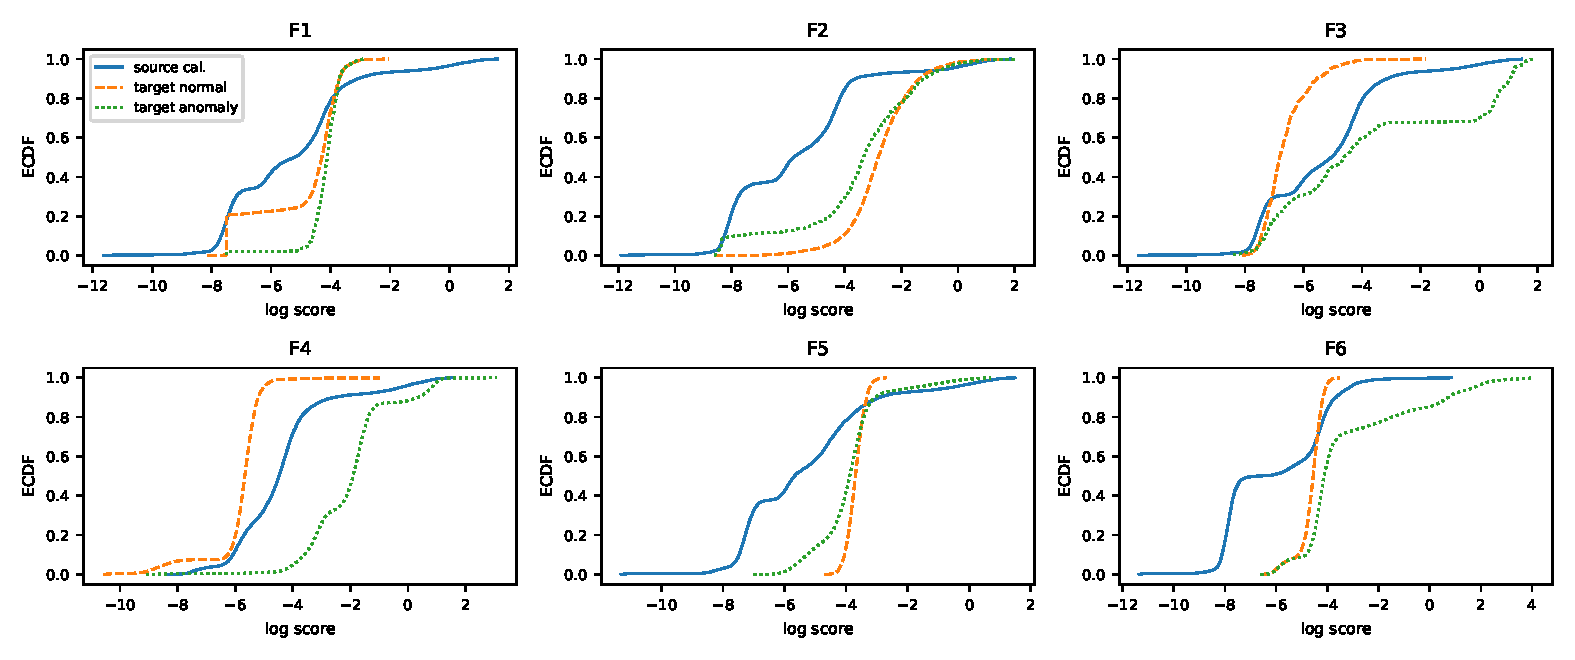
\includegraphics[width=\textwidth]{fig_ecdf.pdf}
\caption{Source-calibration versus target score distributions (log-score ECDFs, seed 0). The inflation numbers have shapes behind them: F2 is a large upward shift with substantial support overlap; F4's target scores sit far below the source-calibration scale (near-disjoint), the regime where static thresholds under-alarm and the relative-gain controller winds up.}
\label{fig:ecdf}
\end{figure*}
 Figure~\ref{fig:operational} shows the inflation bars and exemplar threshold traces: on F2 the static threshold sits orders of magnitude below the target score scale (hence the $0.18$ coverage), while ACI ramps $\qt$ into the target regime; on F6 the trace climbs steadily as the quantile tracks the shifting scores.

The divergence hypothesis, however, does not survive: across folds and seeds, mean band divergence $\Dbar$ and inflation show no reliable association, with Pearson $r\in\{0.13,0.19,0.26,0.30\}$ for $\alphaNom\in\{0.10,0.05,0.20,0.30\}$ ($n{=}18$ per level, all $p>0.22$). An earlier smaller-sample estimate ($n{=}8$) had suggested a borderline correlation; with three seeds it vanishes. Given the small sample, we treat this as evidence against a strong predictive claim rather than a precise null estimate: we keep inflation as a descriptive transfer-cost diagnostic and drop the claim that divergence anticipates it.

\begin{figure}[t]
\centering
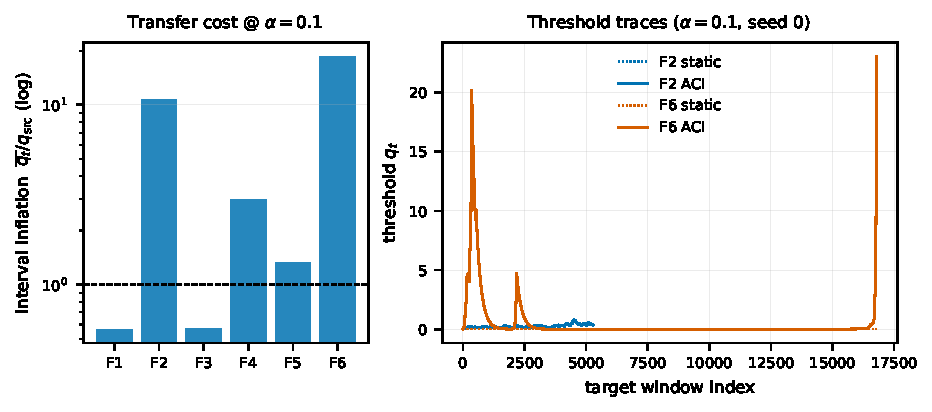
\includegraphics[width=\columnwidth]{fig_operational.pdf}
\caption{Left: threshold inflation $\overline{\qt}/\qsrc$ per fold ($\alphaNom{=}0.10$, log scale). Right: threshold traces on F2 and F6 (static vs ACI, seed 0). Static thresholds are mis-scaled in opposite directions; ACI tracks the target regime.}
\label{fig:operational}
\end{figure}

\subsection{Calibration and Detection Quality Decouple}
\label{sec:decoupling}
AUROC per fold spans the full unusable-to-strong range: $0.63$ (F1), $0.39$ (F2), $0.79$ (F3), $0.99$ (F4), $0.35$--$0.40$ (F5), $0.78$ (F6), with per-seed spread below $0.02$. Two folds rank anomalies \emph{below} chance. We diagnosed both: on F2 and F5, simple feature baselines---window RMS, low-band and high-band energies---also score below $0.5$ (F2: $0.41/0.45/0.37$; F5: $0.36/0.39/0.33$), while the F6 control scores $0.72$--$0.82$ on the same features. The inversion is a property of these datasets under their labeling protocols (fault-labeled periods carry systematically lower amplitude/spectral statistics in this windowing), not a failure unique to our encoder; no repair within our protocol is available, and we therefore \textbf{exclude F2 and F5 from detection-quality claims}. Figure~\ref{fig:decoupling} makes the decoupling explicit: ACI's coverage gap stays near nominal even at AUROC $<0.5$---coverage control is a statement about the threshold, not about the usefulness of the alarms. \textbf{Calibration cannot rescue an anti-correlated ranker}; deployments must audit ranking first (our feature-baseline check is a two-line diagnostic) and only then trust calibrated coverage as a reliability statement.

Detection-side numbers, reported for the four trustworthy folds, are consistent with the coverage picture: false-alarm rates at $\alphaNom{=}0.10$ sit at $85$--$110$ per 1000 normal windows on F1/F2/F4/F5/F6 (F3: $2.3$), and detection delays on F1/F4/F6 are $1$--$2$ windows---roughly $2$--$4$\,min on F1 at 1\,Hz, $2$--$21$\,ms on F4 at 12/128\,kHz, and $5$--$10$\,ms on F6 at 25.6\,kHz---while F5's single run is detected after 49 windows ($\approx 0.13$\,s at the fault-section rate). Window-level AUPRC echoes the ranking picture: it falls below the anomaly prevalence on exactly the two below-chance folds (F2: $0.099$ vs $0.106$; F5: $0.725$ vs $0.729$, where the $73\%$ prevalence dominates the absolute value), while F4 reaches $0.992$. Range-$F_1$ follows the overlapping-run convention (an alarm is credited to a run if it intersects it); the implementation ships with the code. The synthetic F3 study is stable under contamination: AUROC stays within $0.73$--$0.83$ for injection fractions $\{0.05,0.10,0.20,0.40\}$ across seeds.

\begin{figure}[t]
\centering
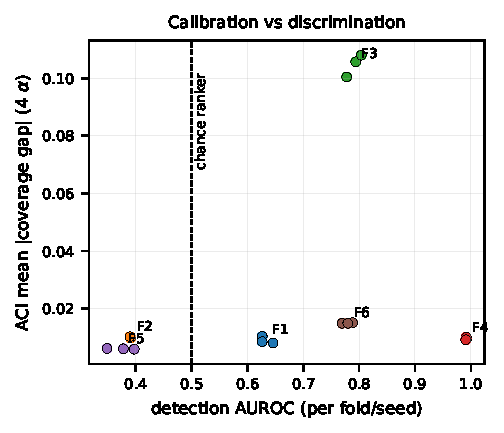
\includegraphics[width=0.82\columnwidth]{fig_decoupling.pdf}
\caption{Calibration versus discrimination: ACI mean coverage gap (four nominal levels) against AUROC for every fold and seed. Below-chance folds (F2, F5) remain coverage-controllable, but their alarms carry no detection utility---an explicit caveat, not a success.}
\label{fig:decoupling}
\end{figure}

\subsection{Contaminated Initialization and Label-Noise Robustness}
\label{sec:robust-init}
Two deployment-side robustness checks (using the first $512$ evaluation windows as the deployment calibration stream). \emph{Contaminated initialization}: if the threshold is initialized from a target segment that contains anomalies, the frozen target-quantile rule degrades exactly as feared---on F4, injecting $10\%$ anomalies into the initialization segment pushes the quantile from $0.07$ to $0.12$ of the source scale (still far too low; the frozen gap stays at $0.89$)---whereas ACI started from the same contaminated value re-converges online: its stream-level gap is $0.018$ on F4, $0.001$ on F2, and $0.006$ on F5, essentially independent of contamination level, at the cost of a slightly longer warm-up (F6's first-$1{,}000$-window gap rises from $0.048$ to $0.067$ at $10\%$ contamination; F3, whose evaluation window is shortest at $1{,}072$ windows, converges slowest). \emph{Label noise}: neither ACI nor NA-ACI uses label information, so symmetric label flips affect evaluation metrics only. At $5$/$10$/$20\%$ flip rates the ACI coverage gap stays at $0.022$/$0.021$/$0.018$, the NA-ACI gap moves from $0.024$ to $0.039$, and static thresholds remain unusable ($0.17$--$0.19$); ranking quality degrades gracefully (mean AUROC $0.64\to 0.58$). Calibration reliability under noisy supervision thus follows the decoupling caveat of Section~\ref{sec:decoupling}: the threshold controller is label-free and stays calibrated; only our ability to \emph{measure} detection quality depends on labels.

\subsection{Calibration Conclusions Are Not Encoder-Specific}
\label{sec:alt-scores}
To test whether the calibration findings depend on our neural encoder, we repeated the comparison on folds F1/F4/F6 with two non-neural score producers: PCA reconstruction (32 components on flattened windows) and a Mahalanobis distance on 16-dimensional band-energy features. Table~\ref{tab:alt} reports mean coverage gaps across the four nominal levels. Static calibration fails for these producers as well---including both failure directions \emph{within} the feature-based producer (F4 over-alarms at coverage $0.06$; F6 never alarms at $0.000$)---while ACI restores gaps to at most $0.011$ in all six producer--fold combinations, even when the producer's ranking is below chance (F1 Mahalanobis, AUROC $0.47$). The calibration layer is agnostic to score provenance, and the decoupling caveat of Section~\ref{sec:decoupling} applies equally to classical detectors.

We further evaluate a \emph{zero-shot time-series foundation model} as an external score producer: Chronos-bolt-small \cite{chronos2024}, scored by its $32$-step forecast residuals (context $224$; median quantile; $4{,}000$ stratified evaluation windows per fold, same splits and injection protocol). Table~\ref{tab:chronos} reports the outcome. The pattern replicates in full: static calibration fails on every fold and in both directions (mean gaps $0.066$--$0.571$); ACI restores gaps to $0.009$--$0.048$; NA-ACI improves further where the budget defect bites (F3: $0.048\!\to\!0.035$, F6: $0.028\!\to\!0.014$; F4 range-$F_1$ $0.27\!\to\!0.39$ with $\kappa{=}3$). Two findings stand out. First, Chronos-bolt ranks anomalies \emph{below chance on the same two folds} as our encoder (F2 AUROC $0.34$, F5 $0.32$), which strongly supports reading the inversion as a dataset/label property rather than an encoder artifact. Second, our $78$K-parameter reconstruction encoder matches or exceeds the zero-shot foundation model on AUROC in all six folds (e.g., F3 $0.79$ vs.\ $0.65$, F4 $0.99$ vs.\ $0.94$), consistent with recent evidence that generic foundation models are not automatically superior on shifted industrial series \cite{freqmatters2025,foundational2025}.

\begin{table}[t]
\caption{Zero-shot Chronos-bolt-small external score producer (forecast-residual scores; 4{,}000 stratified windows per fold). Static fails both ways; ACI restores coverage; NA-ACI tracks the budget defect. AUROC below $0.5$ on F2/F5 matches our encoder---a data/label property, not an encoder artifact.}
\label{tab:chronos}
\centering
\small
\resizebox{\columnwidth}{!}{%
\begin{tabular}{lcccccc}
\toprule
Fold & AUROC & Static gap & ACI gap & NA-ACI gap & R-$F_1$ ACI & R-$F_1$ NA \\
\midrule
F1 & 0.63 & 0.124 & 0.032 & 0.037 ($\kappa{=}5$) & 0.09 & 0.10 \\
F2 & 0.34 & 0.571 & 0.015 & 0.041 ($\kappa{=}5$) & 0.13 & 0.13 \\
F3 & 0.65 & 0.139 & 0.048 & 0.035 ($\kappa{=}5$) & 0.30 & 0.30 \\
F4 & 0.94 & 0.066 & 0.009 & 0.006 ($\kappa{=}5$) & 0.27 & 0.39 \\
F5 & 0.32 & 0.324 & 0.012 & 0.012 ($\kappa{=}5$) & 0.25 & 0.28 \\
F6 & 0.74 & 0.098 & 0.028 & 0.014 ($\kappa{=}5$) & 0.37 & 0.40 \\
\bottomrule
\end{tabular}}
\end{table}

\begin{table}[t]
\caption{Mean coverage gap over four nominal levels for non-neural score producers (static vs.\ ACI). ACI restores coverage in every combination; static fails, including in both directions within the Mahalanobis producer.}
\label{tab:alt}
\centering
\small
\resizebox{\columnwidth}{!}{%
\begin{tabular}{lccc}
\toprule
Producer & F1 & F4 & F6 \\
\midrule
PCA reconstruction (static / ACI)   & 0.154 / \textbf{0.002} & 0.153 / \textbf{0.004} & 0.163 / \textbf{0.011} \\
Mahalanobis band (static / ACI)     & 0.546 / \textbf{0.004} & 0.798 / \textbf{0.002} & 0.838 / \textbf{0.003} \\
\bottomrule
\end{tabular}}
\end{table}

\subsection{Comparison with Rival Cross-Domain Detectors (Mechanism-Level)}
\label{sec:rivals}
Because the official codebases of CICADA \cite{cicada2025} and DACAD \cite{dacad2024} target different benchmarks, we reimplement their core mechanisms under our six-fold protocol and label the comparison accordingly: a \emph{DACAD-style} scorer (anomaly injection + discriminative head + source--target moment alignment) and a \emph{CICADA-style} scorer (four reconstruction experts over source groups with divergence-based expert weighting). Table~\ref{tab:rivals} reports ranking quality and calibration. Three observations. First, the calibration result is universal: static thresholds fail for both rivals on every fold (mean gaps $0.037$--$0.499$, including DACAD-style F2 at $0.037$ and CICADA-style F2 at $0.499$), ACI restores them to $0.001$--$0.101$, and NA-ACI helps where the budget defect bites (CICADA-style F3 gap $0.101\!\to\!0.059$; F4 range-$F_1$ $0.24\!\to\!0.72$). Second, ranking quality of the rivals is unstable across domains---DACAD-style ranges from AUROC $0.26$ (F4) to $0.85$ (F3), and CICADA-style from $0.32$ (F5) to $0.99$ (F4)---so neither is a reliable default. Third, no scorer dominates: our plain encoder matches the best rival on F1/F4/F6 and trails on F2/F3/F5, while every scorer's ranking swings across folds (ours $0.37$--$0.99$, DACAD-style $0.26$--$0.85$, CICADA-style $0.32$--$0.99$)---supporting calibration as the first-order problem for deployment, with ranking left fold-dependent.

\begin{table}[t]
\caption{Mechanism-level rival comparison (6 folds). AUROC per scorer; mean coverage gap static\,$\to$\,ACI; range-$F_1$ (mean over levels) for ACI and NA-ACI. Static fails for both rivals; ACI restores; rival rankings are unstable across folds. Best per-row AUROC in bold.}
\label{tab:rivals}
\centering
\small
\resizebox{\columnwidth}{!}{%
\begin{tabular}{lcccccc}
\toprule
 & \multicolumn{3}{c}{AUROC} & \multicolumn{2}{c}{Gap (static$\to$ACI)} & R-$F_1$ \\
\cmidrule(lr){2-4}\cmidrule(lr){5-6}
Fold & Ours & DACAD* & CICADA* & DACAD* & CICADA* & NA gain \\
\midrule
F1 & \textbf{0.63} & 0.60 & 0.62 & .065$\to$.003 & .075$\to$.006 & --- \\
F2 & 0.39 & \textbf{0.49} & 0.35 & .037$\to$.003 & .499$\to$.010 & --- \\
F3 & 0.79 & \textbf{0.85} & 0.84 & .155$\to$.093 & .155$\to$.101 & 0.59 (k5) \\
F4 & 0.99 & 0.26 & \textbf{0.99} & .064$\to$.002 & .158$\to$.006 & 0.24$\to$0.72 \\
F5 & 0.37 & \textbf{0.59} & 0.32 & .076$\to$.002 & .238$\to$.004 & 0.26$\to$0.27 \\
F6 & 0.78 & 0.53 & \textbf{0.78} & .143$\to$.001 & .133$\to$.011 & 0.26$\to$0.34 \\
\bottomrule
\end{tabular}}
\end{table}

\subsection{Runtime, Memory, and Negative Controls}
\label{sec:neg-controls}
The calibration layer is cheap: across all folds, training takes $\sim$70\,s, target scoring at most $0.41$\,s, and one ACI update costs $0.6$--$0.8\,\mu$s, with $26$\,MB peak GPU memory (Table~\ref{tab:runtime}). The thresholding mechanisms differ negligibly in cost. For completeness we record the negative controls from the predecessor study: spectral-invariance, relation-consistency, and band-saliency losses, low-rank test-time adaptation, and divergence-based source gating each changed range-$F_1$ by at most $2.2\%$ across four folds, and encoder identity (plain vs.\ regularized vs.\ gated) moves calibration coverage by at most $0.002$---which is why this paper studies the calibration layer rather than detector architecture.

\begin{table}[t]
\caption{Per-run cost (one fold, one seed; RTX 3060 Ti). ACI update latency measured over all evaluation windows and nominal levels.}
\label{tab:runtime}
\centering
\small
\resizebox{\columnwidth}{!}{%
\begin{tabular}{lccccc}
\toprule
 & Train (s) & Score (s) & Update ($\mu$s) & Peak mem (MB) & Params \\
\midrule
Value & $\sim$70 & $\leq$0.41 & 0.6--0.8 & 26 & $\sim$78\,K \\
\bottomrule
\end{tabular}}
\end{table}
